\documentclass{standalone}
\usepackage{tikz,amsmath,graphicx}
\usepackage[update,verbose=false]{epstopdf}
\usepackage[version=3]{mhchem}
\graphicspath{{./figs/}}
\newlength{\tikzunit}

\begin{document}
%\begin{figure}[h]
%    \centering
    \setlength{\tikzunit}{\textwidth/20}
    \begin{tikzpicture}[scale=1, x=\tikzunit,y=\tikzunit]
        \node(0,0) {};
        \draw[step= .5,color=gray,thin,dashed](-10, -5) grid ( 10,  5);
        \draw[step=1.0,color=gray]            (-10, -5) grid ( 10,  5);
        \draw[step=5.0,color=black]           (-10, -5) grid ( 10,  5);
        \draw(-10.0, 2.0) node[right]{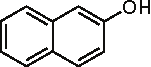
\includegraphics[width=16\tikzunit]{scheme1.pdf}};
    \end{tikzpicture}
%    \caption{Reaction scheme}
%    \label{fig:struct2} 
%\end{figure}
\end{document}
